\chapter{Projekt}

\section{Indledning} 
I dette projekt vil vi kigge nærmere på en lydsekvens, hvor en mand læser højt fra en bog (Tale). Vi vil analysere signalet ved at splitte det op i nogle intervaller, og derefter kigge på eventuelle forskelle. \\Desuden vil vi inddrage endnu en lydsekvens, hvor en mand skælder ud med en hævet stemme (Tale 2). \\De to signaler vil blive sammenlignet og der bliver analyseret eventuelle forskelle og/eller ligheder. 

\section{Analyse af Tale}
På figur 1.1 ses hele talen plottet. Talen er delt op i 6 intervaller af 10 sekunder. Som det blev beskrevet i indledningen, så er denne lydsekvens repræsenteret ved oplæsning fra en bog, og derfor synes der ved første øjekast også en stor lighed mellem de forskellige intervaller. Amplituden i hver af de 6 intervaller svinger mellem -0.18 og 0.18 volt, og generelt er det svært at få øje på markante og forskelle på denne figur.

\begin{figure}[H]
	\centering
	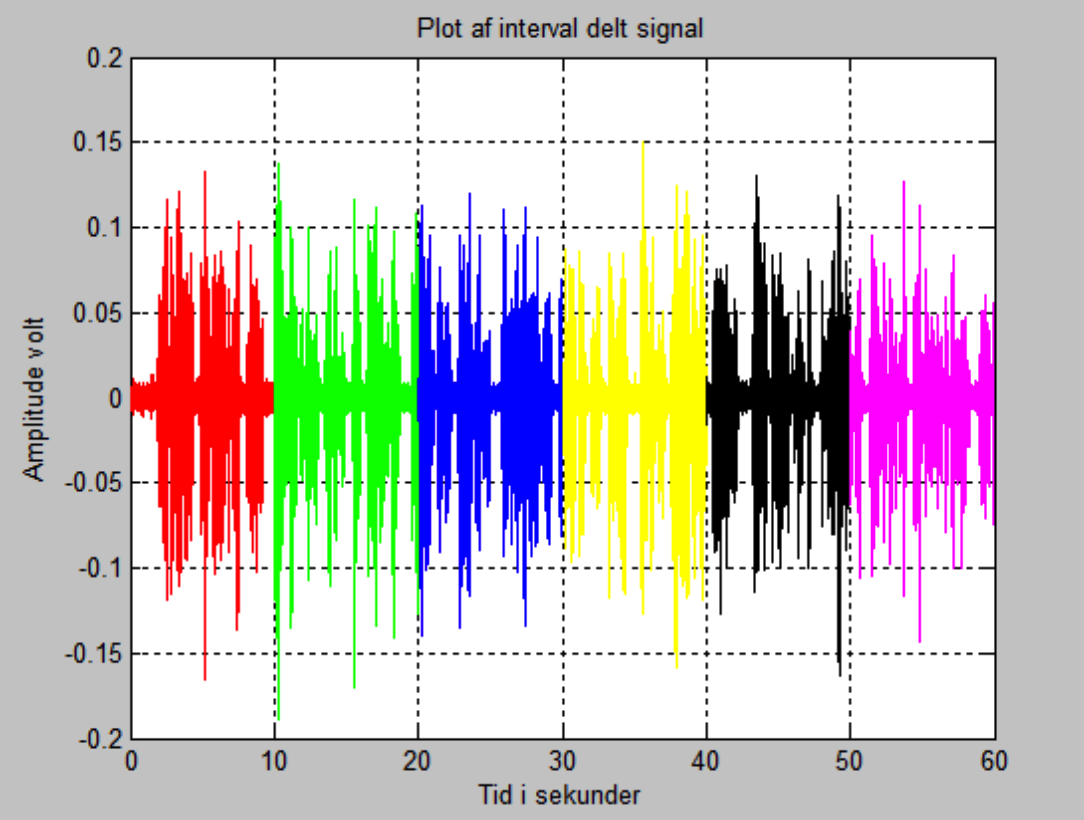
\includegraphics[width=0.8\textwidth]{Figur/Snip20151201_5}
	\caption{Plot af talen}
\end{figure}

Der laves FFT af de forskellige intervaller af talen, da der ønskes at undersøges om der er forskelig på frekvensspektrumet i gennem talen. På de efterfølgende figur 1.2 til 1.7 ses plottet af amplitude, hvor frekvens er hen ad x-aksen og størrelsen dB op ad y-aksen. 


\begin{figure}[H]
	\centering
	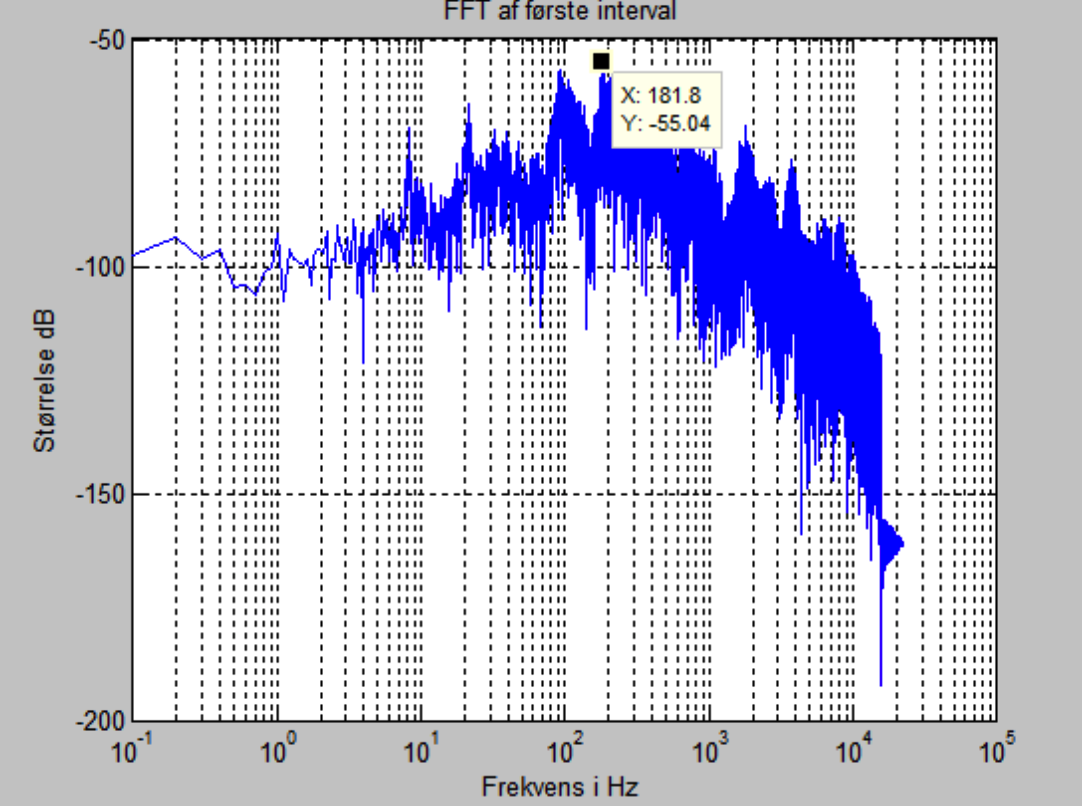
\includegraphics[width=0.8\textwidth]{Figur/Snip20151201_6}
	\caption{Plot af første interval}
\end{figure}

\begin{figure}[H]
	\centering
	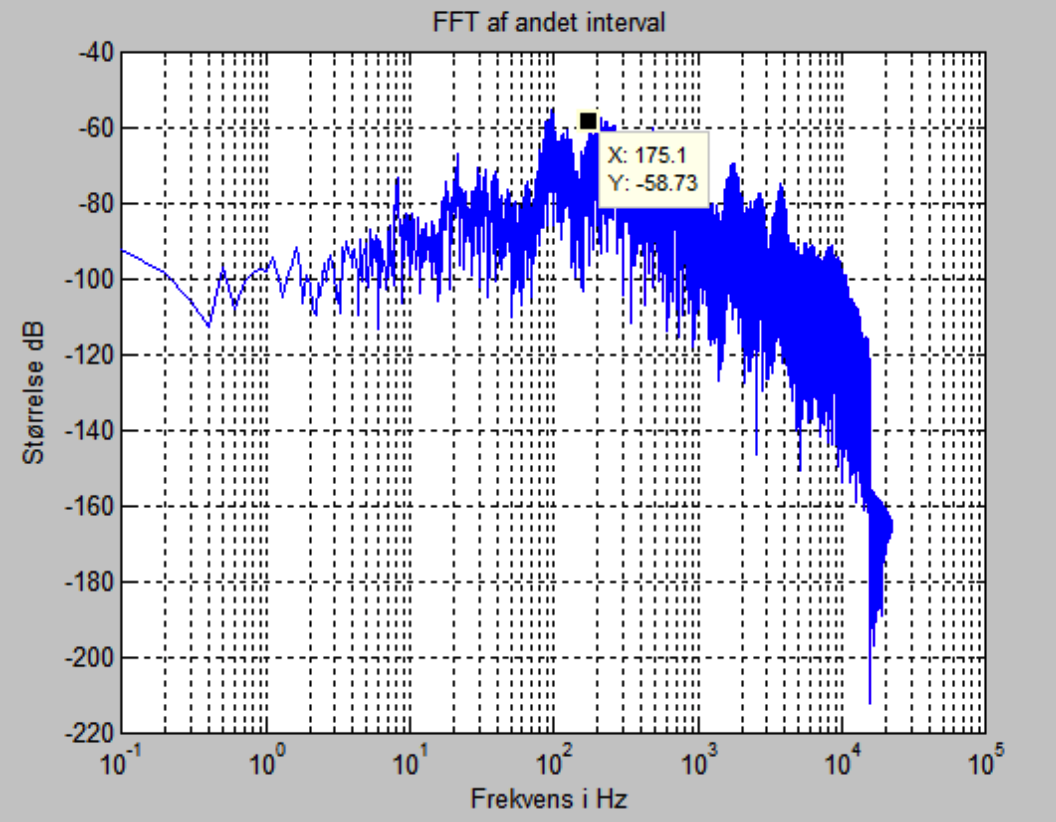
\includegraphics[width=0.8\textwidth]{Figur/Snip20151201_7}
	\caption{Plot af andet interval}
\end{figure}

\begin{figure}[H]
	\centering
	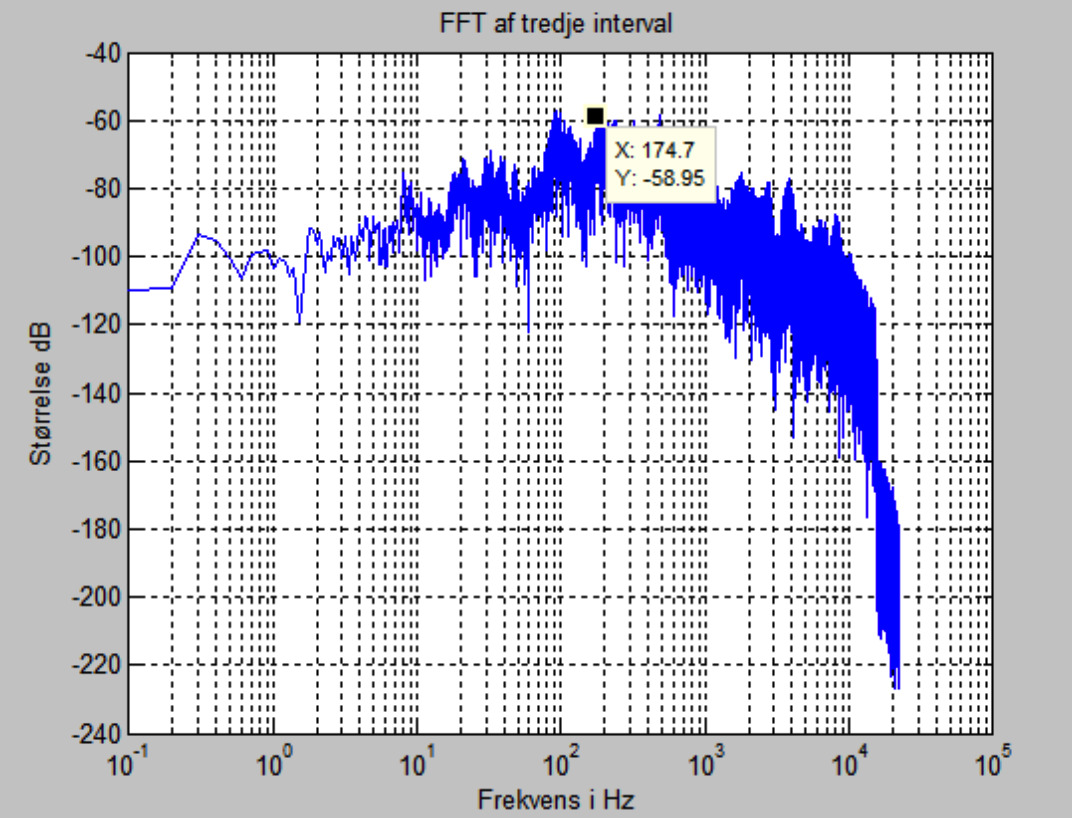
\includegraphics[width=0.8\textwidth]{Figur/Snip20151201_9}
	\caption{Plot af tredje interval}
\end{figure}

\begin{figure}[H]
	\centering
	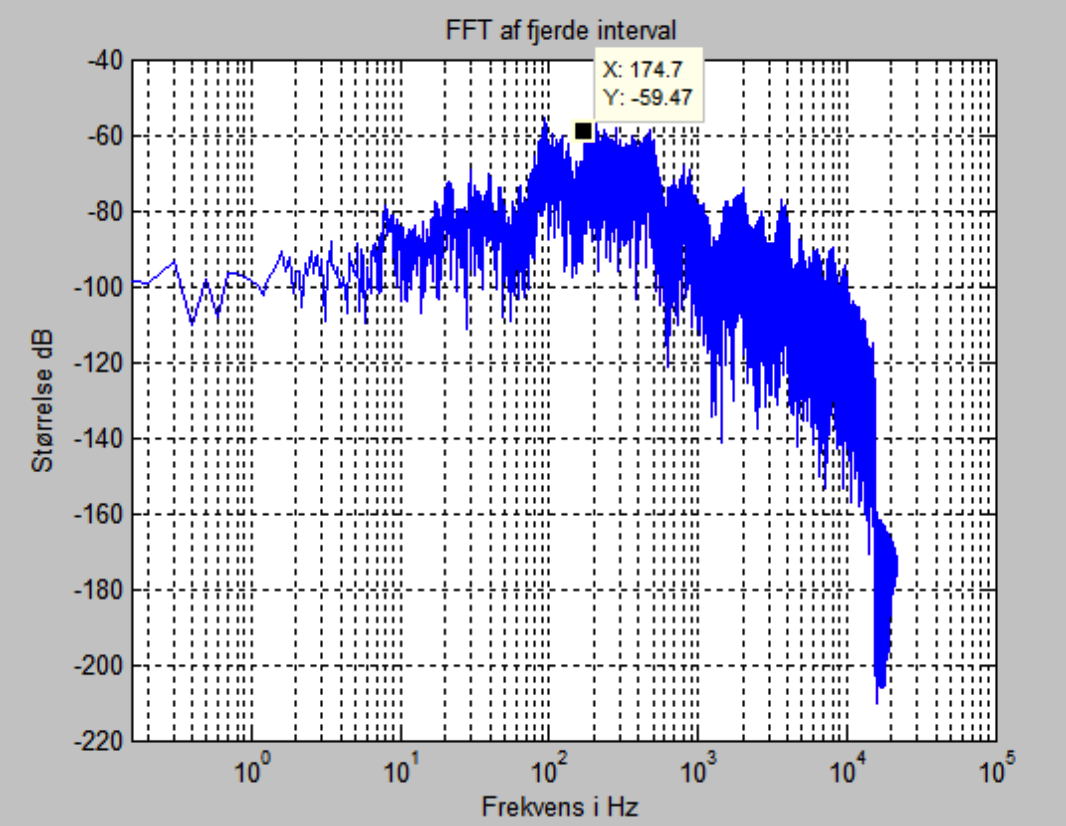
\includegraphics[width=0.8\textwidth]{Figur/Snip20151201_10}
	\caption{Plot af fjerde interval}
\end{figure}

\begin{figure}[H]
	\centering
	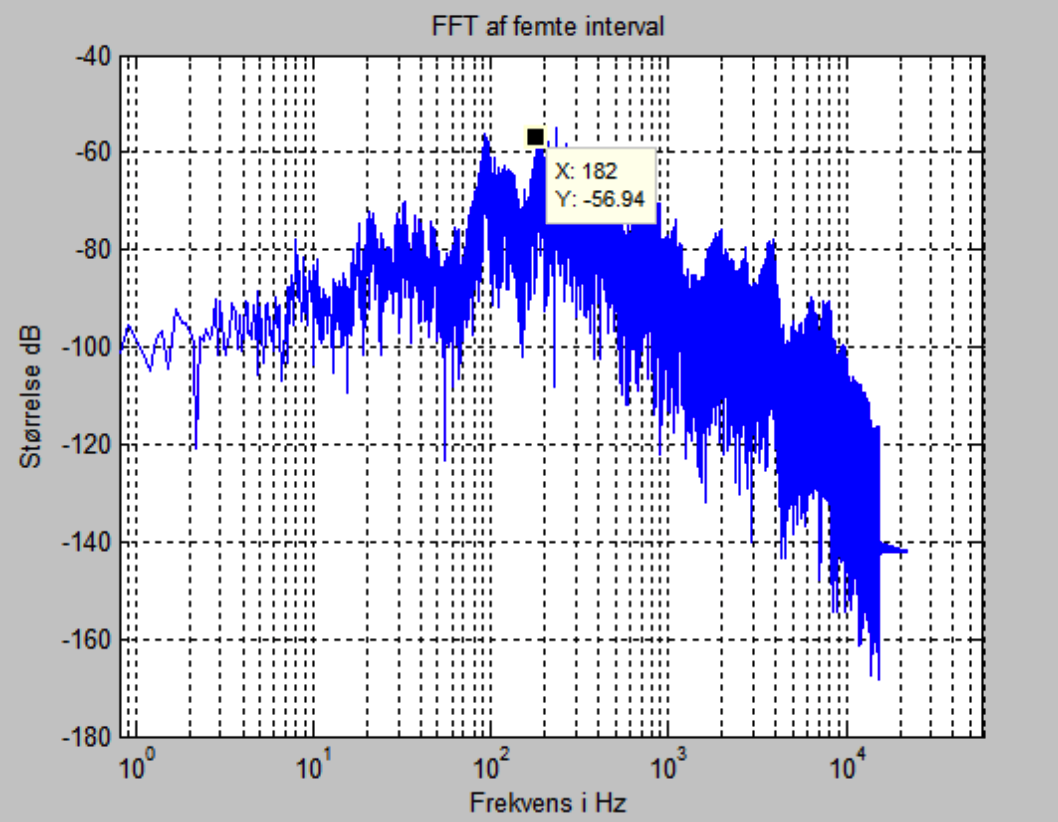
\includegraphics[width=0.8\textwidth]{Figur/Snip20151201_11}
	\caption{Plot af femte interval}
\end{figure}

\begin{figure}[H]
	\centering
	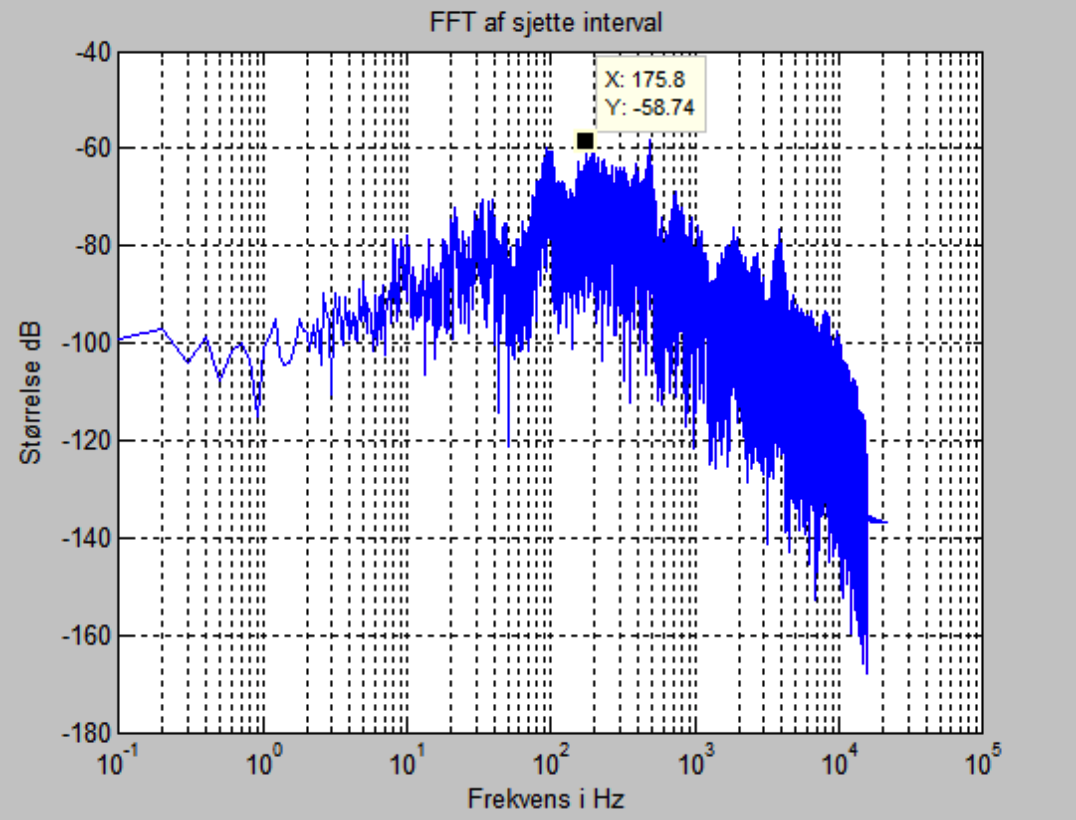
\includegraphics[width=0.8\textwidth]{Figur/Snip20151201_12}
	\caption{Plot af sjette interval}
\end{figure}

Der ses at plottene ser meget ens ud samt at de spænder ud over ca. de samme frekvenser. Dette stemmer overens med Figur 1.1, hvor det ses at intervallerne også er meget ens. En forklaring på det, er at oplæsningen er overvejende monotont, og der er ikke de store ændringer i både lydstyrke og tonelejet. 

\section{Sammenligning af tale og tale 2}
Vi vil gerne se nærmere på om der er en forskel i frekvensen, når man taler på forskellige måder. Vi har valgt, at tage udgangspunkt i oplæsning fra en bog og fra én mand der skælder ud. Vi vil vha. en analyse af frekvensspektret i frekvensdomænet se på, hvorvidt de to signaler adskiller sig fra hinanden, og hvis de gør, hvordan adskiller de sig så fra hinanden?

\begin{figure}[H]
	\centering
	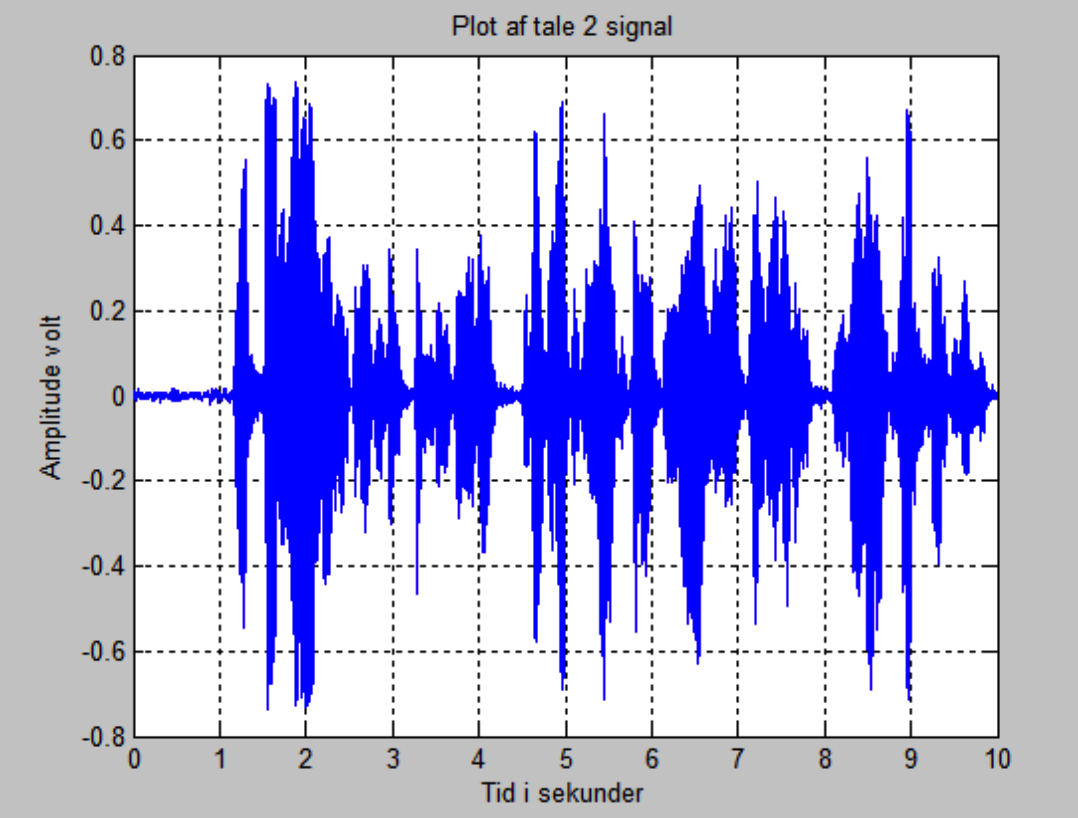
\includegraphics[width=0.8\textwidth]{Figur/Snip20151201_13}
	\caption{Plot af tale 2}
\end{figure}
På figur 1.8 ses et plot af tale 2, som varer 10 sekunder. Det ses på plottet at nogle af de højeste amplituder, ligger ved omkring 0.6-0.8 volt. Det er derved tydeligt at se, at amplituden er højere ved tale 2 end ved oplæsningen, se figur 1.9. Det stemmer overens med, at når man hæver stemmen og tonelejet, så øges amplituden.

\begin{figure}[H]
	\centering
	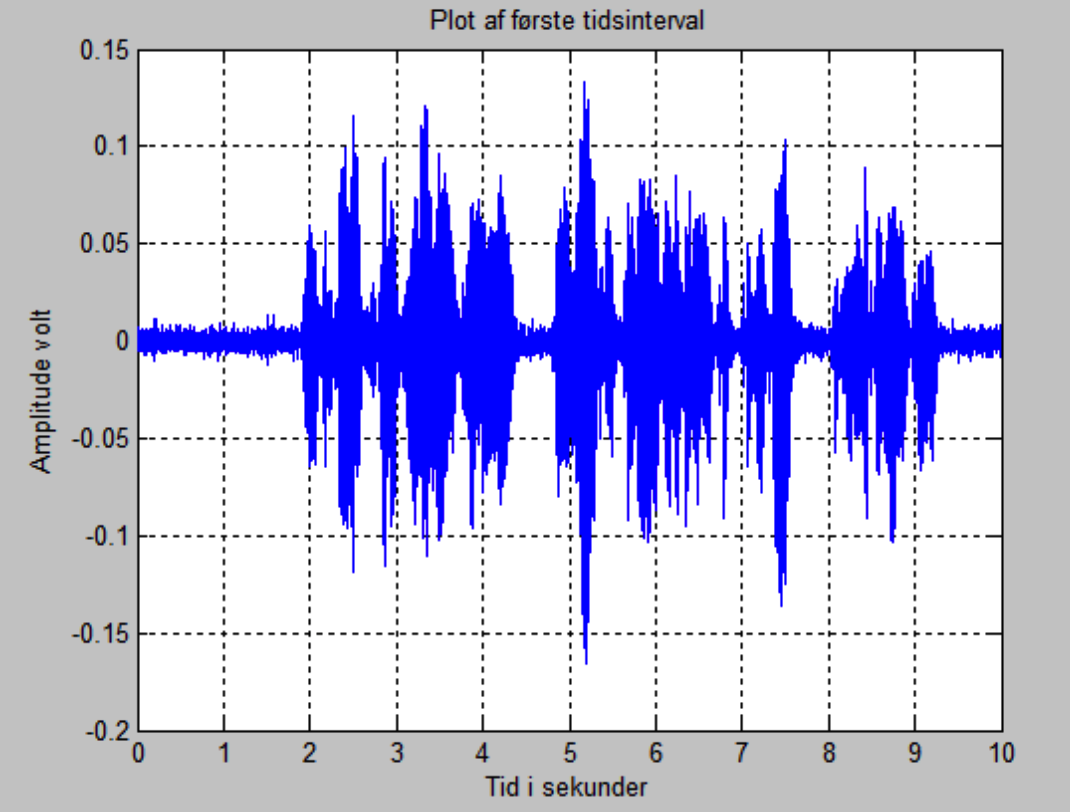
\includegraphics[width=0.8\textwidth]{Figur/Snip20151201_16}
	\caption{Plot af det første interval}
\end{figure}

På figur 1.10 ses plottet af tale 2 i frekvensdomænet. Det ses at frekvensspektrumet har rykket sig til højre - altså frekvenserne er blevet højere. Dette giver også god mening, da der her bliver skældt ud. 

\begin{figure}[H]
	\centering
	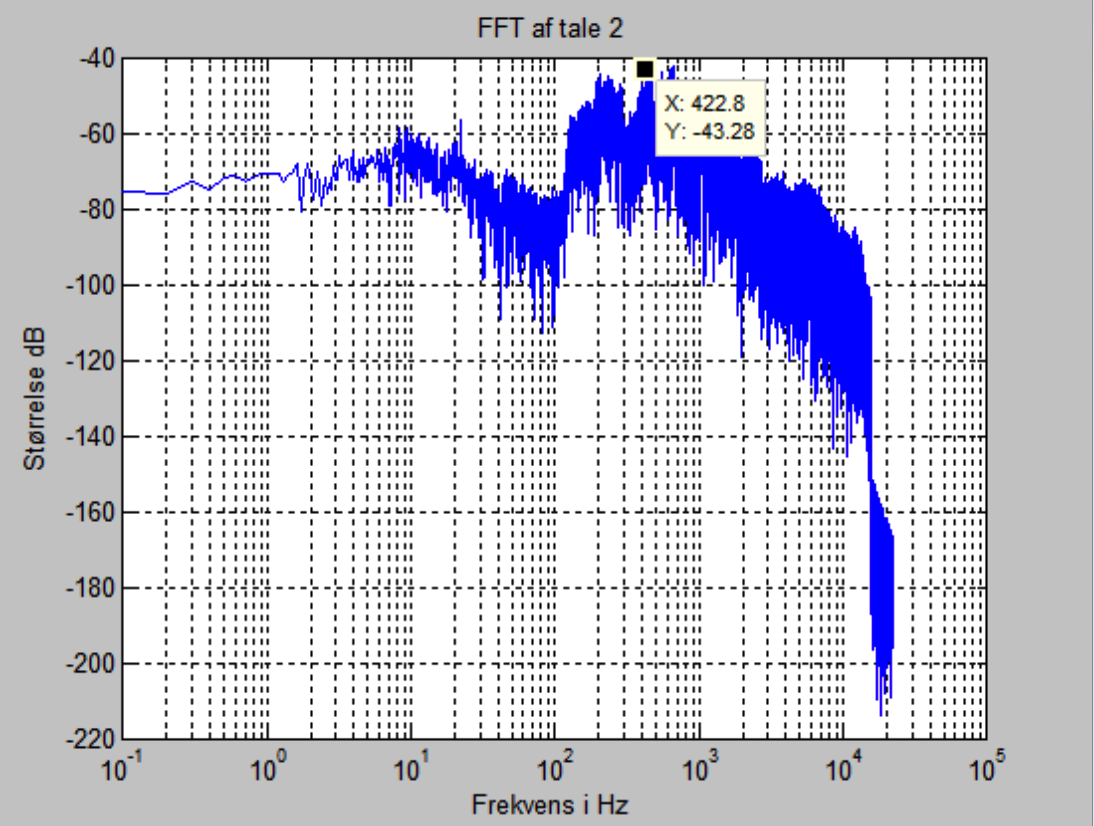
\includegraphics[width=0.8\textwidth]{Figur/Snip20151201_14}
	\caption{Plot af tale 2 FFT}
\end{figure}


\section{Lavpas filtring af talen}
Der ønskes at lavpas filtere de første 10 sekunder af talen så meget, at det ikke længere giver mening, det der bliver sagt. 

\begin{figure}[H]
	\centering
	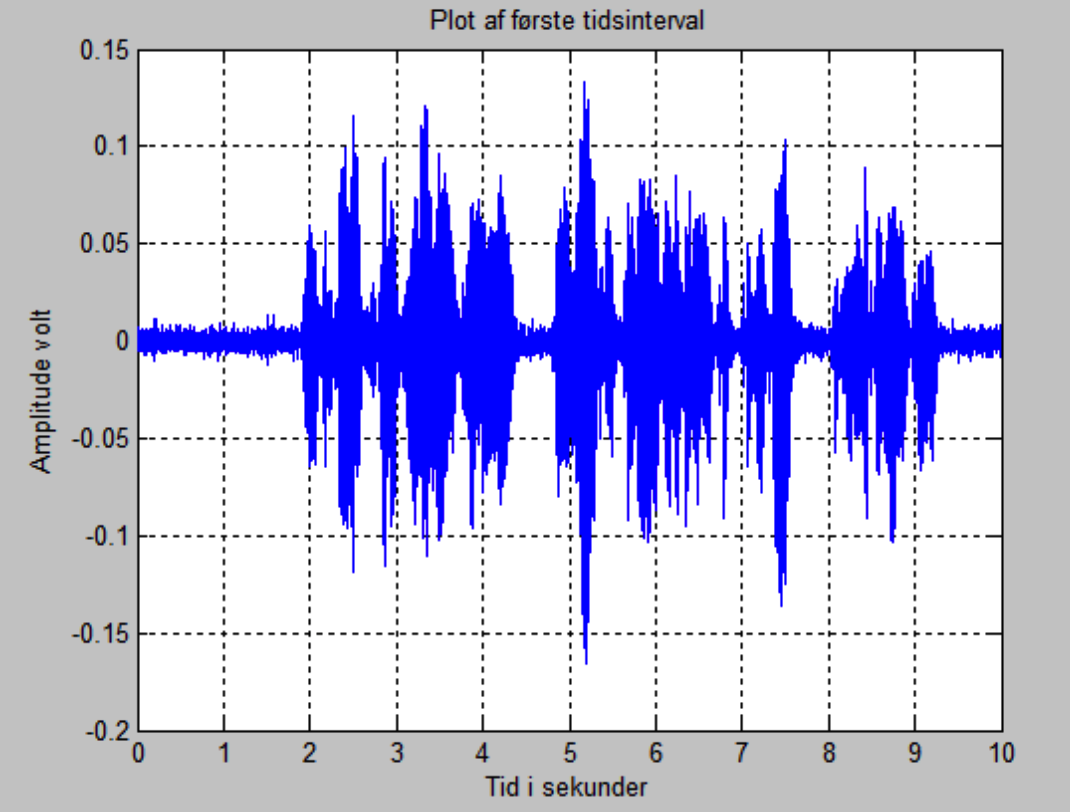
\includegraphics[width=0.8\textwidth]{Figur/Snip20151201_16}
	\caption{Plot af det første interval}
\end{figure}

På figur 1.11 har vi plottet det første interval af talen. Det vil sige de første 10 sekunder af oplæsningen. Det er plottet i tidsdomænet med amplitude i volt som y-akse, og med tiden i sekunder som x-akse. Vi plotter og arbejder med dette tidsinterval, for at filtrere det med et lavpasfilter og sammenligne bagefter. 


\begin{figure}[H]
	\centering
	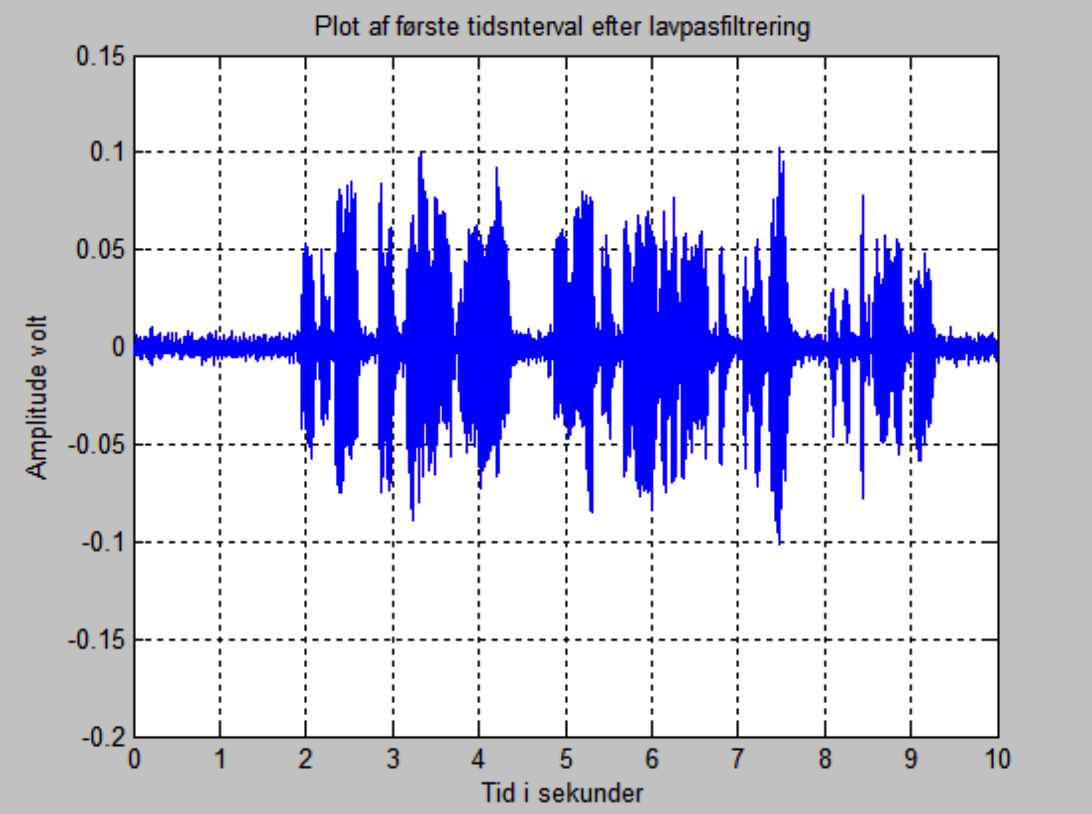
\includegraphics[width=0.8\textwidth]{Figur/Snip20151201_18}
	\caption{Plot af det første interval efter lavpas filtering}
\end{figure}

På figur 1.12 ses det første tidsinterval efter det er filtreret med et lavpasfilter. Lavpasfiltret er lavet som et FIR-filter i MatLab med en orden på 1000. Vi laver denne filtrering for at finde ud af hvilken værdi knækfrekvensen skulle være, for at vi ikke kunne høre og forstå, hvad der bliver sagt i talen. Vi startede altså med en knækfrekvens på 2000 Hz, og hørte om vi kunne forstå lydklippet. Herefter kørte vi knækfrekvensen længere og længere ned, indtil vi ramte 500 Hz. Ved 500 Hz kunne vi ikke længere høre tydeligt, hvad der bliver sagt i talen.
\\ 
\\ 

Vi brugte også lavpasfiltreret på tale 2, hvor der bliver skældt ud. Vi gik ud fra samme fremgangsmåde som ved første tale. Da vi ramte en knækfrekvens på 500 Hz var det rimeligt utydeligt, men sammenlignet med tale 1, var det dog bedre. Der var nogle specifikke udbrud, der var nemme at høre. Det er udbrud som ".. FANDEN..." og andre. Det kan skyldes flere faktorer. For det første er det et ord, der er nemt at genkende. Derudover er det værd at tænke over, at både længden af stemmebåndet kan have betydning, samt hvor højt man snakker, og hvor tæt på mikrofonen man er. 
\\ 
\\

Vi har også plottet faserne for de forskellige intervaller af talen og tale 2 - men vi har ikke medtaget dem, da der ikke kunne siges noget interesant om dem.  












